 \documentclass[11pt,a4paper,onecolumn]{article}
% \documentclass[options]{class}
% Example: \documentclass[11pt,twoside,a4paper]{article} 10 pt is by default.
% !TeX root = ./Sup_info.tex
\setlength{\columnsep}{1cm}
 

\usepackage[T1]{fontenc}       % Use modern font encodings
% \usepackage[version=3]{mhchem} % Formula subscripts using \ce{}
\usepackage{graphicx}
\usepackage[a4paper,top=2cm, bottom=2.5cm, left=2.5cm, right=2.5cm]{geometry}
% \usepackage{authblk} % For affiliation. This package is not preinstalled.
\graphicspath{{./sup_info/}}
\newcommand*\commentauthor[1]{\textbf{{\textit{#1}}}}
\newcommand*\me[1]{\ensuremath{\bar{#1}\,}}
\newcommand*\chem[1]{\ensuremath{\mathrm{#1}}}

\newcommand*{\affaddr}[1]{#1} % No op here. Customize it for different styles.
\newcommand*{\affmark}[1][*]{\textsuperscript{#1}}
\newcommand*{\email}[1]{\texttt{#1}} % These three commands are for author affilations.

\linespread{1.3} % Line spacing. 1.3 means one-and-a-half spacing.

\begin{document}

%\author{
%Biswajit Pradhan, Sebastiaan Van Mulken, Xueyan Miao, Gerard Canters, Michel Orrit\\\affaddr{Huygens-Kamerlingh Onnes Laboratory, Leiden University, 2300 RA Leiden, Netherlands}\\\email{orrit@physics.leidenuniv.nl}
%}

\date{\vspace{1ex}} % Exclude date in the title.
%\affiliation
 %\affil{Huygens-Kamerlingh Onnes Laboratory, Leiden University, 2300 RA Leiden, Netherlands} % This is only useful for authblk package.
 %\email{orrit@leidenuniv.nl}
\title{\textbf{Single azurin redox switching}\\ \vspace{3ex} Supplementary Information \vspace{3ex}}
\maketitle
\tableofcontents
\pagebreak
%%%%%%%%%%%%%%%METHODS AND FIGURES%%%%%%
\section{Protein synthesis and labeling}
\subsection{Protein synthesis}
Azurin (wild type) from Pseudomona aeruginosa was expressed in E. Coli and purified as described before \cite{kamp1990purification}. BL21 E.coli was transformed with PGK22 plasmid that has gene for azurin expression. The cells were cultured in luria broth (LB) medium. Then the cells were harvested and resuspended in 20 \% (w/v) sucrose solution in Tris pH 8 buffer containing 1 mM EDTA.Then the solution was centrifuged at 8000 rpm and the supernatant was collected. Copper sulfate was added to the solution for insertion into the active site of azurin. The unwanted proteins were precipitated by addition of acetic acid until pH 4. Again the turbid solution was centrifuged to separate azurin that remained in the supernatant. The azurin solution was loaded on a CM Sepharose fast flow column and elution was performed in an Akta purifier (GE Healthcare) with a pH gradient from 4 to 6.9 in 50 mM ammonium acetate. Fractions containing azurin collected and reduced with sodium dithionite. At this moment the solution both zinc and copper azurin. The azurins were putified in a DEAE sepharose column by a salt gradient of 0 to 50 mM NaCl in Tris pH8 buffer. Fractions containing copper azurin and zinc azurin collected and concentrated separately. The purity of the samples were checked by sodium dodecyl sulphate (SDS)-polyacrylamide gel electrophoresis (PAGE) and UV/Vis spectroscopy (Cary 50 spectrophotometer, Varian Inc., Agilent Technologies, USA). The azurins appeared on SDS gel page at \~14 kDa. Both zinc and copper azurin showed a characteristic peak at \~290 nm while Cu azurin showed an additional broad absorption peak at 620 nm as can be seen in figure S\ref{SIfig: switching} when oxidized. The ratio $O.D_{628 nm}/O.D_{280}$ for Cu azurin was 0.56 which indcated that all the azurin molecules had a Cu atom. The concentrated protein was stored at $-80^0 C$ until further use.
\subsection{Fluorescent labeling}
The labeling protocol was based on the previous work \cite{nicolardi2012topdown}. ATTO 655 NHS-ester was bought from ATTO-TEC GmbH. The buffer containing azurin was replaced with HEPES pH 8.3 and all the amine containg impurities were removed. A mixture of 200 $\mu$M azurin and ATTO 655 NHS-ester (ration 1:1) was incubated for 45 min. The NHS-ester group reacts to one of the amine group on the protein. The unreacted dyes were removed by a HiTrap desalting column. The labeled protein was concentrated in Tris pH 8.5 buffer by centrifusing in a 3 kDa Amicon ultra filter. The labeled protein further purified by an ion exchange chromatography in a 1 mL MonoQ column (GE Health). The different peaks obtained (see figure S\ref{SIfig: peak_sep}) corresponds to the different number and position of the dye on azurin. The peak-III corresponds to the protein labeled at Lysine122 position \cite{nicolardi2012topdown}. This fraction was choosen for our single-molecule experiemnt for the high switching ratio explained later. The same protocol was used for Zn azurin labeling and similar peak separation observed.
%Peak separation
\begin{figure}
  \centering
  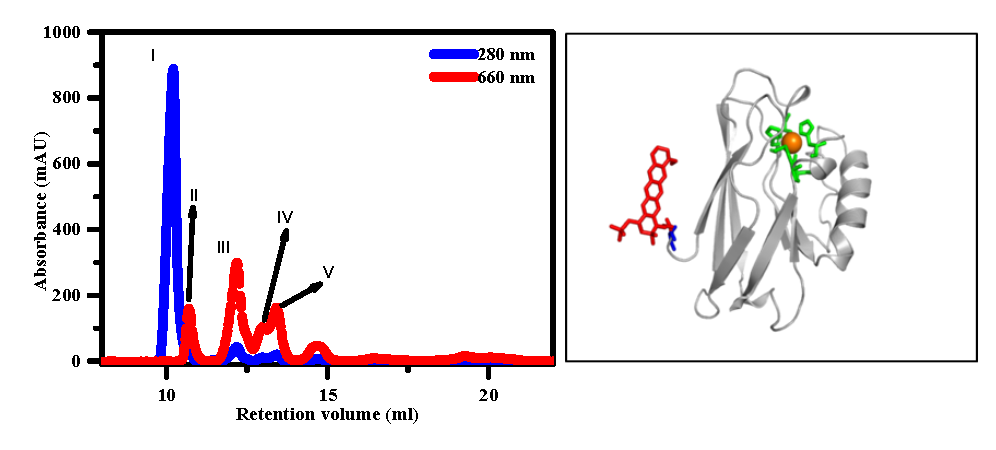
\includegraphics{Figure_SI/peak_separation.eps}
  \makeatletter
  \renewcommand{\fnum@figure}{\figurename~S\thefigure}
  \makeatother
  \caption{Peak separation}
  \label{SIfig: peak_sep}
\end{figure}
%BULK Switching
\begin{figure}
  \centering
  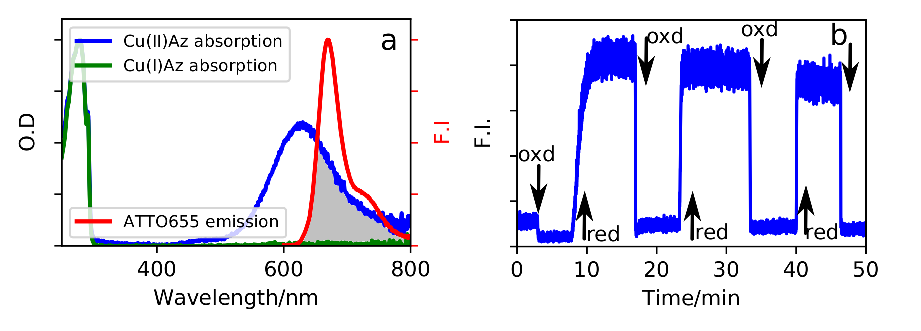
\includegraphics{Figure_SI/spectral_overlap_switching.eps}
  \makeatletter
  \renewcommand{\fnum@figure}{\figurename~S\thefigure}
  \makeatother
  \caption{Bulk switching and spectral overlap}
  \label{SIfig: switching}
\end{figure}
%\section{Time traces}
%lifetime and switching ration from time trace
\begin{figure}
  \centering
  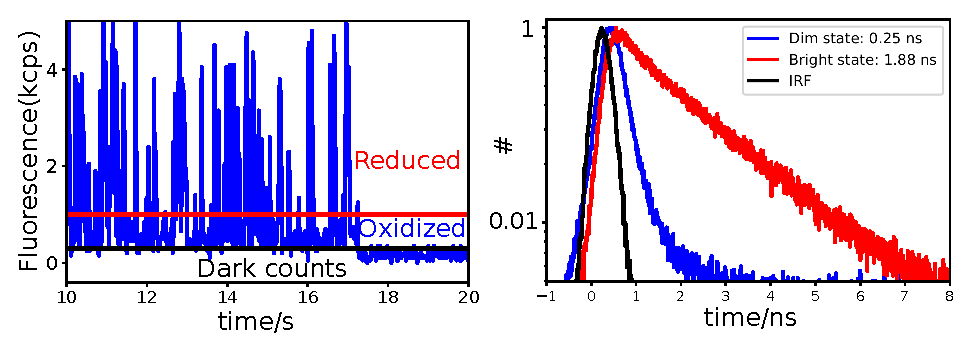
\includegraphics{Figure_SI/lifetime.eps}
  \makeatletter
  \renewcommand{\fnum@figure}{\figurename~S\thefigure}
  \makeatother
  \caption{Switching ratio from single-molecule data. lifetime corresponding to the bright state, dimmer state and instrument response function.}
  \label{SIfig: lifetime}
\end{figure}
%time trace Zn and Cu azurin
\begin{figure}
  \centering
  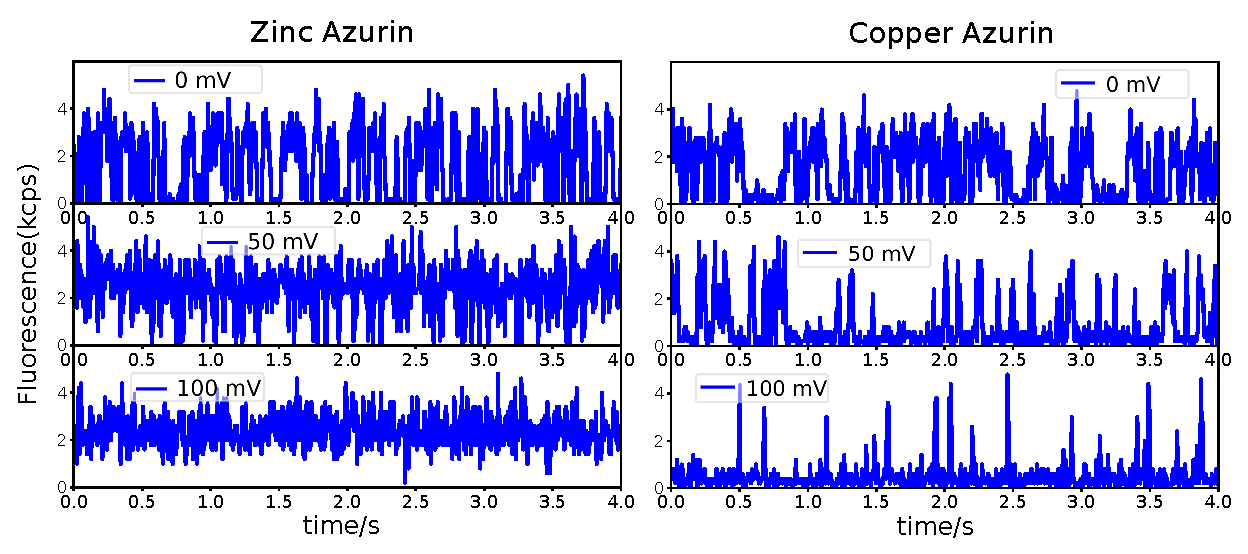
\includegraphics[width=\textwidth,keepaspectratio]{Figure_SI/SI_timetrace_Zn_Cu.eps}
	\makeatletter
	\renewcommand{\fnum@figure}{\figurename~S\thefigure}
	\makeatother
  \caption{Time traces of Zn Azurin (left) and of Cu Azurin(right) labeled with ATTO655 at different potential.  Above 25 mV, Cu-Azurin show swiching in the intensity due to changes in the oxidation state of the Copper metal center and below 25 mV, triplet blinking contributes to the switching as can be seen in the redox inactive Zn-Azurin.}
  \label{SIfig:tracecomparision}
\end{figure}
%mid point potential of ZnAzurin
\begin{figure}
  \centering
  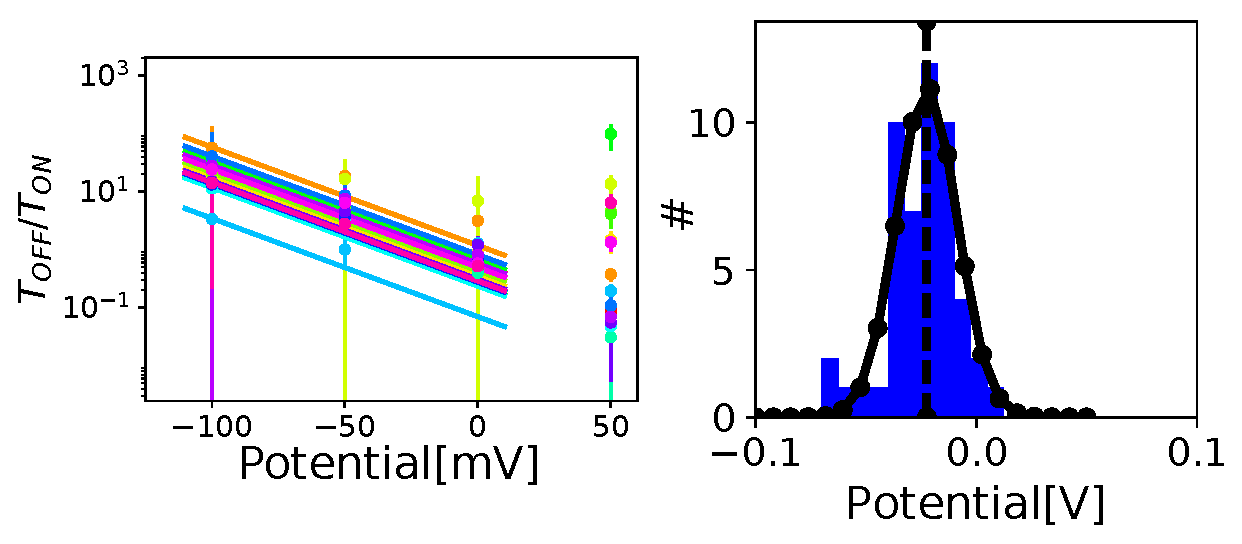
\includegraphics[width=\textwidth,keepaspectratio]{Figure_SI/SI_potential_Zn.eps}
	\makeatletter
	\renewcommand{\fnum@figure}{\figurename~S\thefigure}
	\makeatother
  \caption{\textbf{Zn-AzurinATTO655 blinking.} Ratio between on and off time as a function of applied potential for the same single $ZnAzurin$ molecule. Different color represents different single-molecules. And the line connecting the data points is the Nernst fit for all the data points above 25 mV. The plot in the right is the histogram of midpoint potentials for $51$ molecules with a gaussian fit with center -23 mV with respect to calomel electrode.}
  \label{SIfig:2Dhist_Zn}
\end{figure}
%Slope: Nernst equation
\begin{figure}
  \centering
  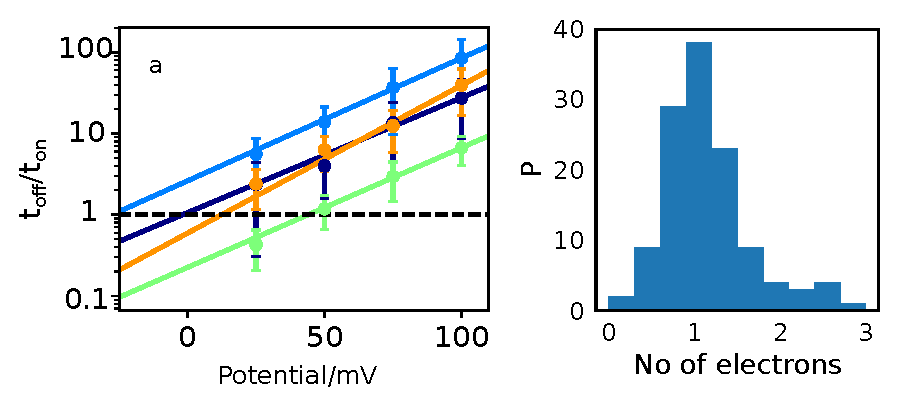
\includegraphics[width=\textwidth,keepaspectratio]{Figure_SI/SI_potential_slope.eps}
	\makeatletter
	\renewcommand{\fnum@figure}{\figurename~S\thefigure}
	\makeatother
  \caption{Fitting with Nernst equation with slope as variable parameters for  (a) Cu-Azurin ATTO655 (b) Zn-Azurin ATTO 655. The corresponding histogram of slopes obtained from the fitting shown in the right.}
  \label{SIfig:potential_slope}
\end{figure}
%Cyclic voltametry: Electrochemical measurement
\begin{figure}
  \centering
  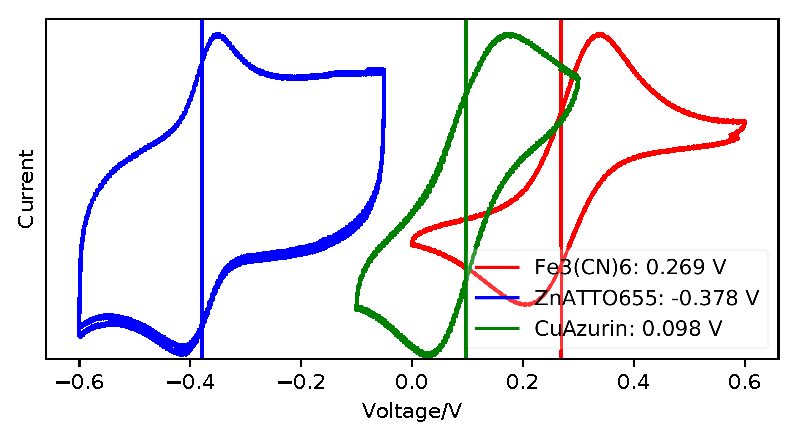
\includegraphics{Figure_SI/cyclic_voltametry.eps}
  \makeatletter
  \renewcommand{\fnum@figure}{\figurename~S\thefigure}
  \makeatother
  \caption{Cyclic voltametry for Cu-Azurin, Pottasium Ferricyanide and ATTO655 attached to ZnAzurin}
  \label{SIfig: cyclic_voltametry}
\end{figure}

\bibliographystyle{ieeetr} % For a list of bibliography styles, see https://www.sharelatex.com/learn/Bibtex_bibliography_styles
\bibliography{Sup_info}
\end{document}